%-----------------------------------------------------------------------------%
\chapter{\babLima}
%-----------------------------------------------------------------------------%

In the previous chapter, the implementation of \verb|JSONField| has been
explained, which includes basic validation of the JSON data. However, the basic
validation only checks the syntax and not the semantics of the data. To
validate the semantics, additional checking can be implemented using Django's
validation features on the application-level, which is demonstrated in this
chapter.

%-----------------------------------------------------------------------------%
\section{Model definitions}
%-----------------------------------------------------------------------------%

Before going through how the validation works, some model definitions are
created for demonstration. The models are defined in a small Django project
with an e-commerce scenario. The project includes two models: \verb|Product|
and \verb|Cart|, both of which utilize \verb|JSONField| in their definitions.

\listing
{Python}
{The \code{Product} model.}
{code:product}
{codes/5-product.py}

The \verb|Product| model shown by \autoref{code:product} represents a product
on an e-commerce website. The \verb|Product| model has an \verb|id| (unique for
each product), a \verb|name|, a \verb|price|, a \verb|stock_qty| (quantity of
the product in stock), and additional \verb|data|. The \verb|data| is stored as
a \verb|JSONField| so that each product can define its own attributes in the
form of a JSON object (\verb|dict| in Python).

\listing
{Python}
{The \code{Cart} model.}
{code:cart}
{codes/5-cart.py}

Meanwhile, the \verb|Cart| model shown by \autoref{code:cart} represents a
shopping cart that is linked to a user and it can hold a list of products. The
list of products is stored in a \verb|JSONField| in the form of a JSON array
(\verb|list| in Python). In addition, the \verb|JSONField| is supplied with two
validators, \verb|validate_cart_products_list| and
\verb|validate_cart_product_ids_exist|. These validators will be used to
validate the data in the list of \verb|products|.

\listing
{Python}
{The \code{add\_product()} method of the \code{Cart} model.}
{code:addproduct}
{codes/5-addproduct.py}

The \verb|Cart| model also has an \verb|add_product()| method to ease the
process of adding a \verb|Product| object to the list of \verb|products|. For
simplicity, the list only holds the \verb|id|, \verb|name|, and \verb|price| of
the \verb|Product| objects, as well as the quantity of each \verb|Product|
object that is added to the cart. The \verb|id| is stored as a hex string
(rather than a \verb|UUID| object) and the \verb|price| is stored as a
\verb|float| (rather than a \verb|Decimal| object) so that the \verb|JSONField|
does not need a custom encoder. Whenever a \verb|Product| is added, the method
iterates through the list of \verb|products| to find the \verb|Product| that
has the same \verb|id| and increments the quantity if it is found, as shown by
lines 15 to 18 of \autoref{code:addproduct}. Otherwise, the data is just
appended to the list, as shown by lines 19 to 26. The list of \verb|products|
will be validated using the validators, as explained in the next section.

%-----------------------------------------------------------------------------%
\section{Validator functions}
%-----------------------------------------------------------------------------%

When defining the fields of a model or a form, Django allows the use of
validators that can be used to validate the data within the field. A validator
is a callable object that takes a value and raises a \verb|ValidationError| if
the value is not valid according to the logic defined by the validator
\cite{django:validators}. To apply validators to a model field or a form field,
they are passed to the field's constructor using the \verb|validators|
argument.

In addition to the built-in validators (e.g. \verb|RegexValidator|,
\verb|EmailValidator|), Django also allows programmers to create their own
validators. A validator is a callable, which means that it can be a function or
an instance of a class that defines the \verb|__call__()| method. In the
previous section, two custom validators are used to validate the list of
\verb|products| (a \verb|JSONField|): \verb|validate_cart_products_list| and
\verb|validate_cart_product_ids_exist|.

\listing
{Python}
{The \code{validate\_cart\_products\_list()} function.}
{code:validatelist}
{codes/5-validatelist.py}

The first validator function is the \verb|validate_cart_products_list()|
function shown by \autoref{code:validatelist}. The function works by checking
whether the \verb|products| value is an instance of \verb|list|. If it is not,
a \verb|ValidationError| is raised. This validator function can be seen as a
basic schema validator for the JSON data that ensures the data is a JSON array.
To validate against a more complex schema, programmers can use a third-party
library such as jsonschema\footnote{\url{https://github.com/Julian/jsonschema}}
or Cerberus\footnote{\url{https://github.com/pyeve/cerberus}} and raise a
\verb|ValidationError| if the library indicates that the data is invalid.

\listing
{Python}
{The \code{validate\_cart\_product\_ids\_exist()} function.}
{code:validateids}
{codes/5-validateids.py}

The second validator function is \verb|validate_cart_product_ids_exist()| that
ensures the \verb|id|s of the \verb|Product| data inside the list of
\verb|products| also exist in the database. To prevent errors while validating
the list of \verb|products|, the validator immediately returns if the
\verb|products| value is not a list, as shown by lines 2 and 3 of
\autoref{code:validateids}. Otherwise, the validator takes the \verb|id|s of
each product in the cart into a list of \verb|product_ids| (line 6).

Then, a query is executed to look for the \verb|Product| objects where the
\verb|id| is in the list of \verb|product_ids| (line 8). To retrieve the
\verb|id|s back as strings (not as \verb|UUID| objects), the \verb|Cast|
function is used to cast the \verb|id| into a \verb|CharField| (lines 9 and
10). The \verb|values_list()| method is used so that the query only retrieves
the \verb|id|s without the other information of the \verb|Product| model (line
11). Line 13 of the listing shows that the set of \verb|product_ids| is
subtracted by the set of \verb|id|s retrieved from the database
(\verb|valid_ids|). If the subtraction results in a non-empty set, that means
the list of \verb|products| contain \verb|Product| information with invalid
\verb|id|s, so a \verb|ValidationError| is raised, as shown by lines 14 to 17
of the listing. As all of the validators have been implemented, they can now be
used to validate the list of \verb|products|.

%-----------------------------------------------------------------------------%
\section{Demonstration}
%-----------------------------------------------------------------------------%

To use the validators, they need to be run manually before saving the model
object, because the method does not run them automatically. To run the
validators, the \verb|clean_fields()| method of the model object should be
called. The method can be called either directly or indirectly by calling the
\verb|full_clean()| method of the model object, which calls
\verb|clean_fields()| as part of its process.

\begin{figure}
	\centering
    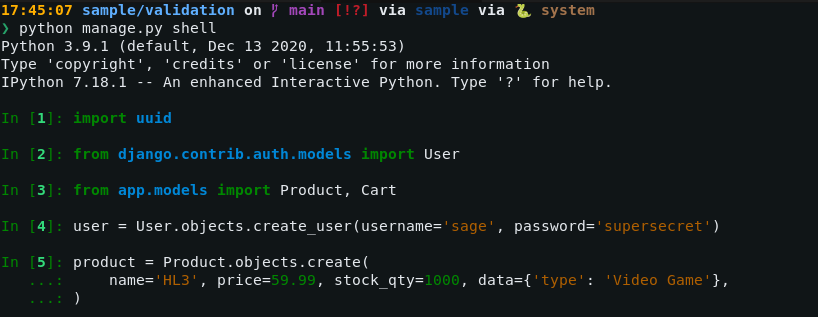
\includegraphics[width=1.00\textwidth]{pics/validation0.png}
	\caption{The initialization for the validation demonstration.}
	\label{fig:validation0}
\end{figure}

Before demonstrating the validators in action, some model objects are created,
as shown by \autoref{fig:validation0}. The first object is a \verb|User| object
that is assigned to the \verb|user| variable, which will be assigned to a
\verb|Cart| object. The second object is a \verb|Product| model object that is
assigned to the \verb|product| variable, which will be added to a \verb|Cart|
object. Both of these objects are created with the \verb|create()| method,
so they are immediately saved to the database. After these objects are created,
the validators are demonstrated below.

\begin{figure}
	\centering
    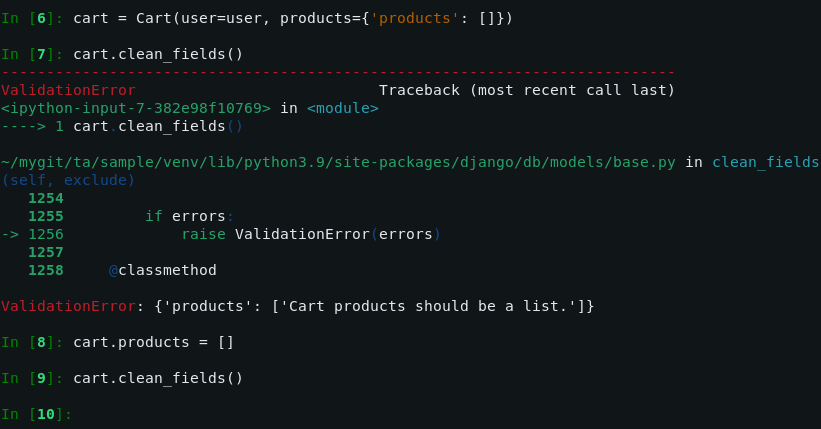
\includegraphics[width=1.00\textwidth]{pics/validation1.png}
	\caption{The \code{validate\_cart\_products\_list()} validator in action.}
	\label{fig:validation1}
\end{figure}

To run the validators before the \verb|Cart| model object is saved to the
database, an instance of the \verb|Cart| class is created (rather than using
the \verb|create()| method). The instance is linked to the \verb|user| created
previously and is initialized with the dictionary \verb|{'products': []}| as
the value for the \verb|products| field. When calling the \verb|clean_fields()|
method, a \verb|ValidationError| is raised, as shown by
\autoref{fig:validation1}. The error message (that comes from the
\verb|validate_cart_products_list| validator) indicates that the
\verb|products| field value should be a \verb|list|, not a dictionary. After
changing the \verb|products| field value to an empty \verb|list| (\verb|[]|),
calling the \verb|clean_fields()| method again does not raise any errors.

\begin{figure}
	\centering
    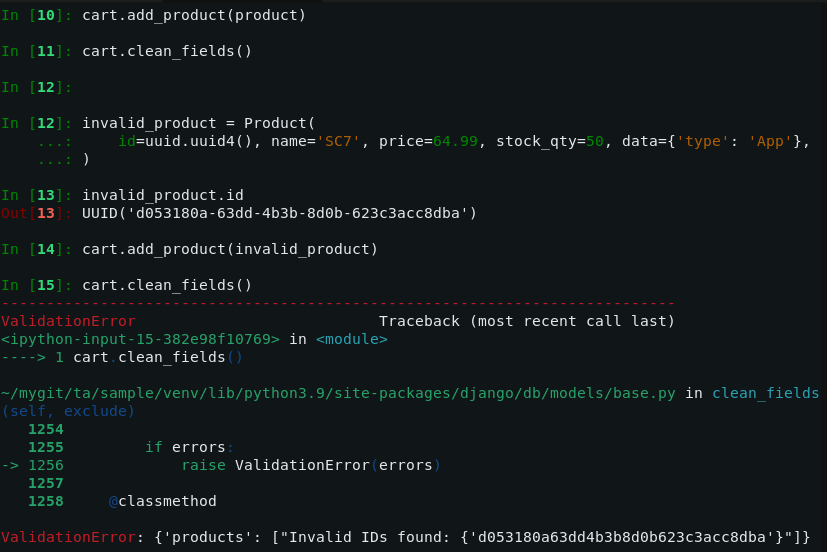
\includegraphics[width=0.90\textwidth]{pics/validation2.png}
	\caption{The \code{validate\_cart\_product\_ids\_exist} validator in action.}
	\label{fig:validation2}
\end{figure}

The next validator is the \verb|validate_cart_product_ids_exist()| function.
Before demonstrating this validator, the previously made \verb|product| object
is added to the \verb|cart|. If the \verb|clean_fields()| method is called, no
error is raised because the \verb|product| exists in the database, as shown by
input 11 of \autoref{fig:validation2}. After that, a new \verb|Product|
instance is created without saving it to the database (input 12). If the
instance is added to the \verb|cart| (input 14) and the \verb|clean_fields()|
method is called, a \verb|ValidationError| is raised (input 15). The error
message indicates that the invalid ID is equal to the new \verb|Product|
instance \verb|id| (input and output 13). The error is raised because the
new instance does not exist in the database yet.

\begin{figure}
	\centering
    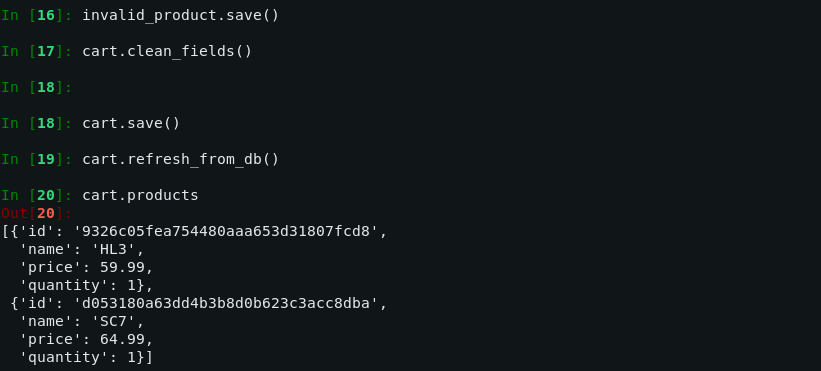
\includegraphics[width=0.90\textwidth]{pics/validation3.png}
	\caption{The \code{Cart} object is saved after passing the validations.}
	\label{fig:validation3}
\end{figure}

If the new \verb|Product| instance is saved, calling the \verb|clean_fields()|
method again does not raise an error, as shown by inputs 16 and 17 of
\autoref{fig:validation3}. As the list of \verb|products| in the \verb|cart|
has been validated, it can now be safely saved to the database. To save the
\verb|Cart| object, the \verb|save()| method is called (input 18). To verify
that the object is successfully saved, the \verb|refresh_from_db()| method is
called (input 19). As shown by input and output 20, the list of \verb|products|
were successfully stored to and retrieved from the database.

In this chapter, JSON data validation for a \verb|JSONField| has been
explained. The validation is implemented by creating custom validator functions
using and supplying them to the field using the \verb|validators| argument to
the field's constructor. To run the validators, the \verb|clean_fields()|
method of the field is called. If the data is not valid, the validators raise
\verb|ValidationError|s, which can be caught to prevent invalid data from being
saved to the database. In the next chapter, the \verb|JSONField| implementation
will be evaluated on multiple database systems.
